\documentclass[10pt]{article}
\usepackage[utf8]{inputenc}
\usepackage[T1]{fontenc}
\usepackage{amsmath}
\usepackage{amsfonts}
\usepackage{amssymb}
\usepackage[version=4]{mhchem}
\usepackage{stmaryrd}
\usepackage{graphicx}
\usepackage[export]{adjustbox}
\graphicspath{ {./images/} }

\title{Gaussian Mixture Models }


\author{Martin Jaggi\\
Last updated on: November 28, 2023}
\date{}


\begin{document}
\maketitle
Machine Learning Course - CS-433

Nov 28, 2023

credits to Mohammad Emtiyaz Khan \& Rüdiger Urbanke

EPFL

\section*{Motivation}
K-means forces the clusters to be spherical, but sometimes it is desirable to have elliptical clusters. Another issue is that, in K-means, each example can only belong to one cluster, but this may not always be a good choice, e.g. for data points that are near the "border". Both of these problems are solved by using Gaussian Mixture Models.

\section*{Clustering with Gaussians}
The first issue is resolved by using full covariance matrices $\boldsymbol{\Sigma}_{k}$ instead of isotropic covariances.

$p(\mathbf{X} \mid \boldsymbol{\mu}, \boldsymbol{\Sigma}, \mathbf{z})=\prod_{n=1}^{N} \prod_{k=1}^{K}\left[\mathcal{N}\left(\mathbf{x}_{n} \mid \boldsymbol{\mu}_{k}, \boldsymbol{\Sigma}_{k}\right)\right]^{z_{n k}}$

\section*{Soft-clustering}
The second issue is resolved by defining $z_{n}$ to be a random variable. Specifically, define $z_{n} \in$ $\{1,2, \ldots, K\}$ that follows a multinomial distribution.

$p\left(z_{n}=k\right)=\pi_{k}$ where $\pi_{k}>0, \forall k$ and $\sum_{k=1}^{K} \pi_{k}=1$

This leads to soft-clustering as opposed to having "hard" assignments.

\begin{center}
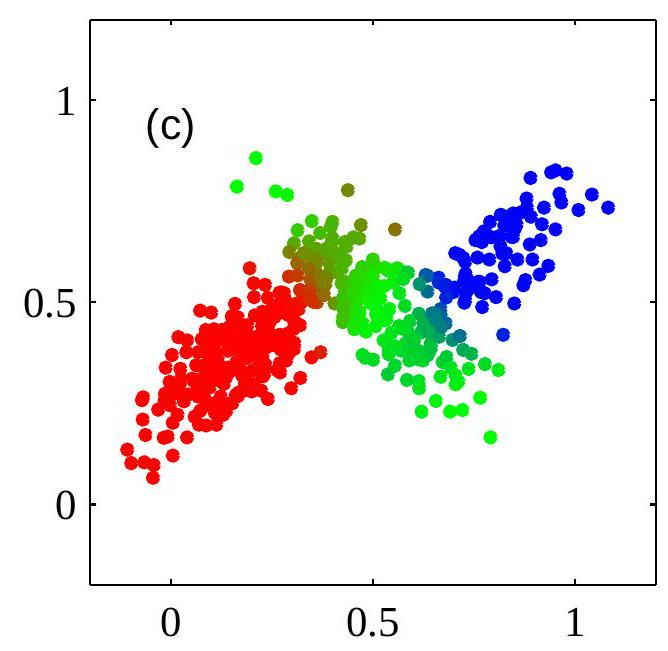
\includegraphics[max width=\textwidth]{2023_12_30_0ee90ffe1a149a681222g-3}
\end{center}

\section*{Gaussian mixture model}
Together, the likelihood and the prior define the joint distribution of Gaussian mixture model (GMM):

$$
\begin{aligned}
& p(\mathbf{X}, \mathbf{z} \mid \boldsymbol{\mu}, \boldsymbol{\Sigma}, \boldsymbol{\pi}) \\
& =\prod_{n=1}^{N} p\left(\mathbf{x}_{n} \mid z_{n}, \boldsymbol{\mu}, \boldsymbol{\Sigma}\right) p\left(z_{n} \mid \boldsymbol{\pi}\right) \\
& =\prod_{n=1}^{N} \prod_{k=1}^{K}\left[\mathcal{N}\left(\mathbf{x}_{n} \mid \boldsymbol{\mu}_{k}, \boldsymbol{\Sigma}_{k}\right)\right]^{z_{n k}} \prod_{k=1}^{K}\left[\pi_{k}\right]^{z_{n k}}
\end{aligned}
$$

Here, $\mathbf{x}_{n}$ are observed data vectors, $z_{n}$ are latent unobserved variables, and the unknown $p a$ rameters are given by $\boldsymbol{\theta}:=$ $\left\{\boldsymbol{\mu}_{1}, \ldots, \boldsymbol{\mu}_{K}, \boldsymbol{\Sigma}_{1}, \ldots, \boldsymbol{\Sigma}_{K}, \boldsymbol{\pi}\right\}$.

\section*{Marginal likelihood}
GMM is a latent variable model with $z_{n}$ being the unobserved (latent) variables. An advantage of treating $z_{n}$ as latent variables instead of parameters is that we can marginalize them out to get a cost function that does not depend on $z_{n}$, i.e. as if $z_{n}$ never existed.

Specifically, we get the following marginal likelihood by marginalizing $z_{n}$ out from the likelihood:

$p\left(\mathbf{x}_{n} \mid \boldsymbol{\theta}\right)=\sum_{k=1}^{K} \pi_{k} \mathcal{N}\left(\mathbf{x}_{n} \mid \boldsymbol{\mu}_{k}, \boldsymbol{\Sigma}_{k}\right)$
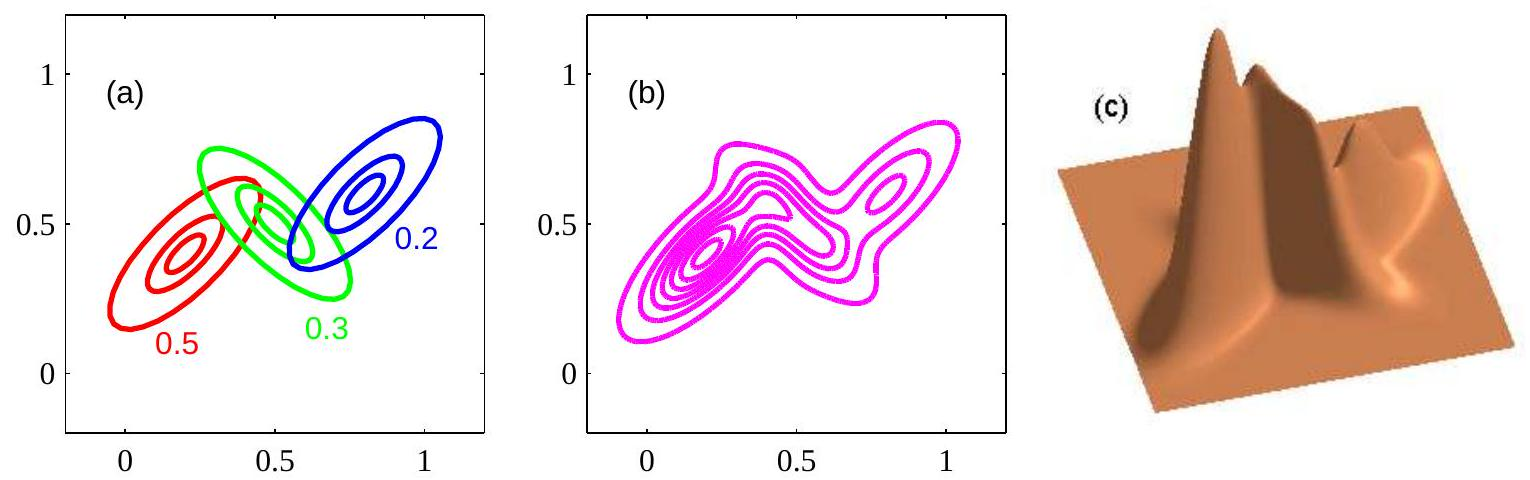
\includegraphics[max width=\textwidth, center]{2023_12_30_0ee90ffe1a149a681222g-4}

Deriving cost functions this way is good for statistical efficiency. Without a latent variable model, the number of parameters grows at rate $\mathcal{O}(N)$. After marginalization, the growth is reduced to $\mathcal{O}\left(D^{2} K\right)$ (assuming $D, K \ll N)$.

\section*{Maximum likelihood}
To get a maximum (marginal) likelihood estimate of $\boldsymbol{\theta}$, we maximize the following:

$$
\max _{\boldsymbol{\theta}} \sum_{n=1}^{N} \log \sum_{k=1}^{K} \pi_{k} \mathcal{N}\left(\mathbf{x}_{n} \mid \boldsymbol{\mu}_{k}, \boldsymbol{\Sigma}_{k}\right)
$$

Is this cost convex? Identifiable?

Bounded?

\begin{center}
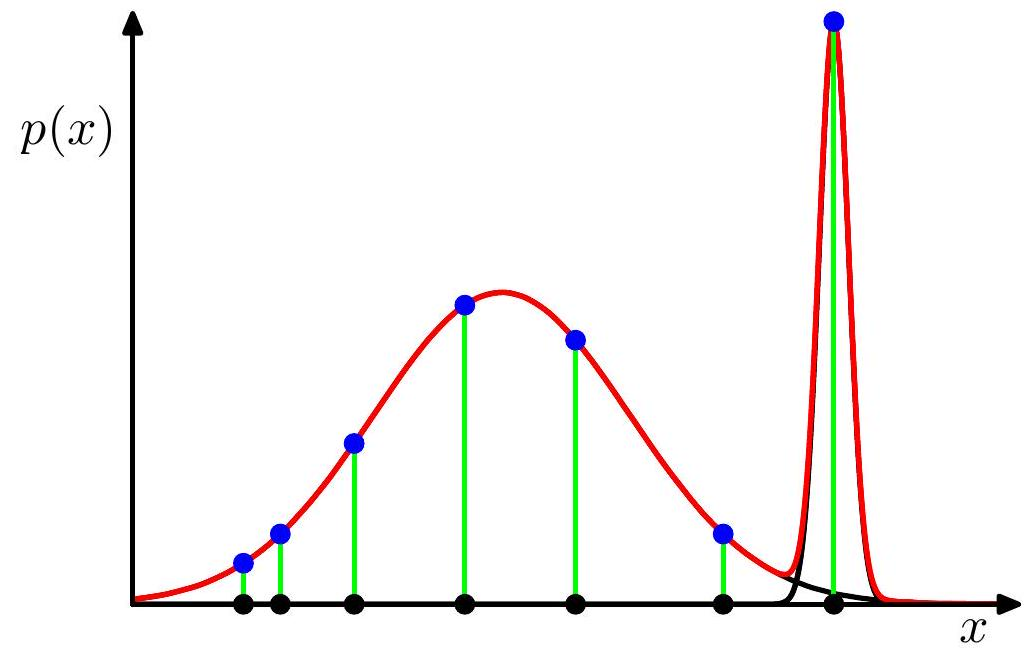
\includegraphics[max width=\textwidth]{2023_12_30_0ee90ffe1a149a681222g-5}
\end{center}


\end{document}